\begin{itemize}
  \item few-shot learning from demonstration and neural program induction
  \item inputs a task specification (e.g. video specification) and recursively decomposes it into finer sub-tasks
  \item Complex manipulation tasks: object sorting, assembly, de-cluttering, etc
  \item NTP interprets a task specification and instantiates a hierarchical policy as a neural program
  \item Task specification can either be a task demonstration recorded as a state-trajectory or even a list of language instructions
  \item NTP generalizes to 3 kinds of variations in task structure: task length, task topology, and task semantics
  \begin{figure}[H]
    \caption{NTP}
    \centering
    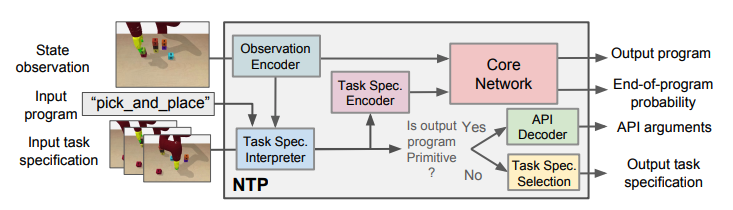
\includegraphics[width=\textwidth]{../../imgs/ntp.png}
  \end{figure}
  \item NTP is a meta-learning algorithm, decomposes final objective into simpler objectives recursively and each subtask is assigned a neural program
  \item NTP extends upon NPI (Neural Programmer-Interpreter)
  \item NPI is a type of neural program induction in, core of NPI is an LSTM which selects at every timestep the next program to run
  \item NTP has three parts: Task Specification Interpreter ($f_{TSI}$), Task Specification Encoder ($f_{TSE}$), and a core network ($f_{CN}$)
  \begin{figure}[H]
    \caption{NTP Algorithm}
    \centering
    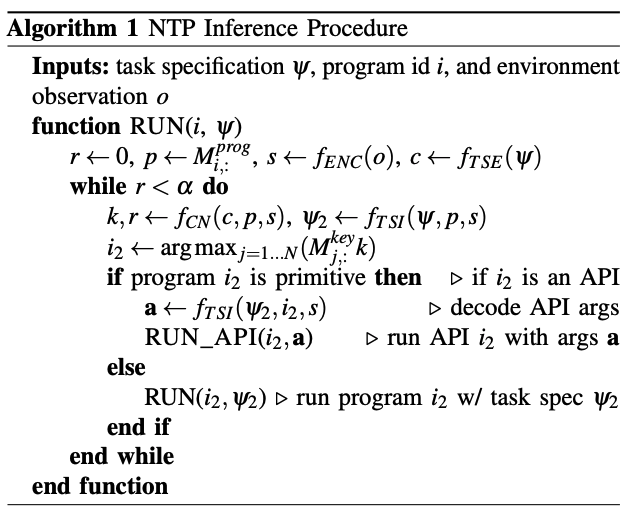
\includegraphics[width=0.5\textwidth]{../../imgs/ntp_algorithm.png}
  \end{figure}
  \item NTP vs NPI: NTP can interpret task specifications and perform hierarchical decomposition, NTP uses APIs as primitive actions and it uses a reactive core network instead of a RNN
  \item APIs are subroutines for learning at an abstract level, APIs take in specific arguments (e.g. object category or end-effector position)
  \item APIs used were move\_to, grip, and release
\end{itemize}